\documentclass[11pt]{article}\usepackage[]{graphicx}\usepackage[]{xcolor}
% maxwidth is the original width if it is less than linewidth
% otherwise use linewidth (to make sure the graphics do not exceed the margin)
\makeatletter
\def\maxwidth{ %
  \ifdim\Gin@nat@width>\linewidth
    \linewidth
  \else
    \Gin@nat@width
  \fi
}
\makeatother

\definecolor{fgcolor}{rgb}{0.345, 0.345, 0.345}
\newcommand{\hlnum}[1]{\textcolor[rgb]{0.686,0.059,0.569}{#1}}%
\newcommand{\hlstr}[1]{\textcolor[rgb]{0.192,0.494,0.8}{#1}}%
\newcommand{\hlcom}[1]{\textcolor[rgb]{0.678,0.584,0.686}{\textit{#1}}}%
\newcommand{\hlopt}[1]{\textcolor[rgb]{0,0,0}{#1}}%
\newcommand{\hlstd}[1]{\textcolor[rgb]{0.345,0.345,0.345}{#1}}%
\newcommand{\hlkwa}[1]{\textcolor[rgb]{0.161,0.373,0.58}{\textbf{#1}}}%
\newcommand{\hlkwb}[1]{\textcolor[rgb]{0.69,0.353,0.396}{#1}}%
\newcommand{\hlkwc}[1]{\textcolor[rgb]{0.333,0.667,0.333}{#1}}%
\newcommand{\hlkwd}[1]{\textcolor[rgb]{0.737,0.353,0.396}{\textbf{#1}}}%
\let\hlipl\hlkwb

\usepackage{framed}
\makeatletter
\newenvironment{kframe}{%
 \def\at@end@of@kframe{}%
 \ifinner\ifhmode%
  \def\at@end@of@kframe{\end{minipage}}%
  \begin{minipage}{\columnwidth}%
 \fi\fi%
 \def\FrameCommand##1{\hskip\@totalleftmargin \hskip-\fboxsep
 \colorbox{shadecolor}{##1}\hskip-\fboxsep
     % There is no \\@totalrightmargin, so:
     \hskip-\linewidth \hskip-\@totalleftmargin \hskip\columnwidth}%
 \MakeFramed {\advance\hsize-\width
   \@totalleftmargin\z@ \linewidth\hsize
   \@setminipage}}%
 {\par\unskip\endMakeFramed%
 \at@end@of@kframe}
\makeatother

\definecolor{shadecolor}{rgb}{.97, .97, .97}
\definecolor{messagecolor}{rgb}{0, 0, 0}
\definecolor{warningcolor}{rgb}{1, 0, 1}
\definecolor{errorcolor}{rgb}{1, 0, 0}
\newenvironment{knitrout}{}{} % an empty environment to be redefined in TeX

\usepackage{alltt}

% Packages for graphics & layout
\usepackage{graphicx}
\usepackage{epstopdf}
\usepackage{caption}
\usepackage{subcaption}
\usepackage{booktabs}
\usepackage[a4paper,margin=0.5in]{geometry}
\usepackage{lipsum}

\usepackage[utf8]{inputenc}
\usepackage{enumitem}

% Packages for math
\usepackage{amsmath}
\usepackage{amsfonts}
\usepackage{amssymb}

% Package for bibliography
\usepackage{natbib}
\usepackage{hyperref}

% listing setup \usepackage{listings}
\usepackage{color} % For syntax highlighting color
\captionsetup{labelfont=bf}
\setlength{\parskip}{0.5\baselineskip}


\title{\textbf{Data Analysis Report}}
\author{Michael V Cumbo}
\date{\today}
\IfFileExists{upquote.sty}{\usepackage{upquote}}{}
\begin{document}

\maketitle

\section{Introduction}
This paper was written in response to the United Auto Workers strike and the SAG-AFTRA strike of 2023. The goal of this paper is to contextualize the state of trade union power in the United States, blending data analysis with a literature review. The data in this paper will contextualize union power in a select number of nation-states, adding perspective to the modes of influence unions have.

\section{Methodology}
\subsection*{Libraries Used in the Analysis}

This analysis utilized several R packages, each contributing unique functions essential for data management, manipulation, visualization, and database interaction. Below is a description of each package and its role in our analysis:

\section*{R Packages Overview}
\begin{enumerate}
    \item \textbf{Tidyverse}
    \begin{itemize}[noitemsep]
        \item Description: An aggregation of several data manipulation packages. Simplifies many aspects of data analysis. Includes packages like \texttt{ggplot2} for data visualization, \texttt{dplyr} for data manipulation, and \texttt{readr} for data import.
        \item Installation: \texttt{install.packages("tidyverse")}
        \item Documentation: \href{https://www.tidyverse.org/}{tidyverse.org}
    \end{itemize}

    \item \textbf{RSQLite}
    \begin{itemize}[noitemsep]
        \item Description: Provides a database interface and SQLite driver for R. Allows for storage, management, and retrieval of large datasets efficiently.
        \item Installation: \texttt{install.packages("RSQLite")}
        \item Documentation: \href{https://cran.r-project.org/web/packages/RSQLite/index.html}{RSQLite on CRAN}
    \end{itemize}

    \item \textbf{DBI}
    \begin{itemize}[noitemsep]
        \item Description: Defines a common interface between R and database management systems. Essential for establishing database connections and executing queries.
        \item Installation: \texttt{install.packages("DBI")}
        \item Documentation: \href{https://cran.r-project.org/web/packages/DBI/index.html}{DBI on CRAN}
    \end{itemize}

    \item \textbf{Ggplot2}
    \begin{itemize}[noitemsep]
        \item Description: Part of the \texttt{tidyverse}, a tool for creating elegant data visualizations in R, based on the Grammar of Graphics.
        \item Installation: \texttt{install.packages("ggplot2")}
        \item Documentation: \href{https://ggplot2.tidyverse.org/}{ggplot2.tidyverse.org}
    \end{itemize}

    \item \textbf{Dplyr}
    \begin{itemize}[noitemsep]
        \item Description: Within the \texttt{tidyverse}, used for data manipulation with verbs like filter, select, mutate, and summarize.
        \item Installation: \texttt{install.packages("dplyr")}
        \item Documentation: \href{https://dplyr.tidyverse.org/}{dplyr.tidyverse.org}
    \end{itemize}

    \item \textbf{Forcats}
    \begin{itemize}[noitemsep]
        \item Description: Part of the \texttt{tidyverse}, designed for handling categorical variables in R. Provides functions for reordering factor levels and more.
        \item Installation: \texttt{install.packages("forcats")}
        \item Documentation: \href{https://forcats.tidyverse.org/}{forcats.tidyverse.org}
    \end{itemize}

    \item \textbf{GGally}
    \begin{itemize}[noitemsep]
        \item Description: An extension of \texttt{ggplot2}, providing additional functions for creating complex multi-plot layouts.
        \item Installation: \texttt{install.packages("GGally")}
        \item Documentation: \href{https://cran.r-project.org/web/packages/GGally/index.html}{GGally on CRAN}
    \end{itemize}

    \item \textbf{Stringr}
    \begin{itemize}[noitemsep]
        \item Description: Also part of the \texttt{tidyverse}, it simplifies working with strings (text data) in R.
        \item Installation: \texttt{install.packages("stringr")}
        \item Documentation: \href{https://stringr.tidyverse.org/}{stringr.tidyverse.org}
    \end{itemize}
\end{enumerate}
\subsection{Data Collection}
Data was sourced from the International Labor Organization, OECD datasets, and Harvard datasets.
\subsection{Data Preparation}

\begin{knitrout}
\definecolor{shadecolor}{rgb}{0.969, 0.969, 0.969}\color{fgcolor}\begin{kframe}
\begin{alltt}
\hlcom{# Initialize an empty list to store plots}
\hlstd{plots_list} \hlkwb{<-} \hlkwd{list}\hlstd{()}
\hlcom{# Loop for 'joined_full_data_set' (Union Density)}
\hlstd{country_focus} \hlkwb{<-} \hlkwd{unique}\hlstd{(joined_full_data_set}\hlopt{$}\hlstd{ref_area)}
\hlkwa{for} \hlstd{(country} \hlkwa{in} \hlstd{country_focus) \{}
  \hlstd{TUD_country} \hlkwb{<-} \hlstd{joined_full_data_set} \hlopt
    \hlkwd{filter}\hlstd{(ref_area} \hlopt{==} \hlstd{country)}

  \hlstd{wrapped_title} \hlkwb{<-} \hlkwd{str_wrap}\hlstd{(}\hlkwd{paste}\hlstd{(}\hlstr{"Time Series of Union Density in"}\hlstd{,}
                                  \hlstd{country,} \hlstr{"(ILOdata)"}\hlstd{),} \hlkwc{width} \hlstd{=} \hlnum{30}\hlstd{)}
  \hlstd{plot} \hlkwb{<-} \hlkwd{ggplot}\hlstd{(TUD_country,} \hlkwd{aes}\hlstd{(}\hlkwc{x} \hlstd{= time,} \hlkwc{y} \hlstd{= `Union Density`))} \hlopt{+}
    \hlkwd{geom_line}\hlstd{(}\hlkwc{color} \hlstd{=} \hlstr{"#00BFC4"}\hlstd{,} \hlkwc{size} \hlstd{=} \hlnum{1.2}\hlstd{)} \hlopt{+}
    \hlkwd{labs}\hlstd{(}
      \hlkwc{title} \hlstd{= wrapped_title,}
      \hlkwc{x} \hlstd{=} \hlstr{"Year"}\hlstd{,}
      \hlkwc{y} \hlstd{=} \hlstr{"Union Density (in %)"}
    \hlstd{)} \hlopt{+}
    \hlkwd{theme_minimal}\hlstd{(}\hlkwc{base_size} \hlstd{=} \hlnum{14}\hlstd{)} \hlopt{+}
    \hlstd{tstheme} \hlopt{+}
    \hlkwd{scale_y_continuous}\hlstd{(}\hlkwc{breaks} \hlstd{= scales}\hlopt{::}\hlkwd{pretty_breaks}\hlstd{(}\hlkwc{n} \hlstd{=} \hlnum{10}\hlstd{),}
                       \hlkwc{labels} \hlstd{= scales}\hlopt{::}\hlkwd{label_number}\hlstd{(}\hlkwc{auto} \hlstd{=} \hlnum{TRUE}\hlstd{))}
  \hlstd{plots_list[[}\hlkwd{paste}\hlstd{(}\hlstr{"Union_Density"}\hlstd{, country)]]} \hlkwb{<-} \hlstd{plot}
\hlstd{\}}
\hlcom{# Loop for 'cbcr' data frame}
\hlkwa{for} \hlstd{(country} \hlkwa{in} \hlkwd{unique}\hlstd{(cbcr}\hlopt{$}\hlstd{ref_area)) \{}
  \hlstd{cbcr_country} \hlkwb{<-} \hlstd{cbcr} \hlopt
    \hlkwd{filter}\hlstd{(ref_area} \hlopt{==} \hlstd{country)}

  \hlstd{wrapped_title} \hlkwb{<-} \hlkwd{str_wrap}\hlstd{(}\hlkwd{paste}\hlstd{(}\hlstr{"Collective Bargaining Coverage Over Time in"}\hlstd{,}
                                  \hlstd{country,} \hlstr{"(ILOdata)"}\hlstd{),} \hlkwc{width} \hlstd{=} \hlnum{30}\hlstd{)}

  \hlstd{plot} \hlkwb{<-} \hlkwd{ggplot}\hlstd{(cbcr_country,} \hlkwd{aes}\hlstd{(}\hlkwc{x} \hlstd{= time,} \hlkwc{y} \hlstd{= obs_value))} \hlopt{+}
    \hlkwd{geom_line}\hlstd{(}\hlkwc{color} \hlstd{=} \hlstr{"#2ca02c"}\hlstd{,} \hlkwc{size} \hlstd{=} \hlnum{1.2}\hlstd{)} \hlopt{+}
    \hlkwd{geom_point}\hlstd{(}\hlkwc{color} \hlstd{=} \hlstr{"#d62728"}\hlstd{,} \hlkwc{size} \hlstd{=} \hlnum{2}\hlstd{,} \hlkwc{alpha} \hlstd{=} \hlnum{0.7}\hlstd{)} \hlopt{+}
    \hlkwd{labs}\hlstd{(}
      \hlkwc{title} \hlstd{= wrapped_title,}
      \hlkwc{x} \hlstd{=} \hlstr{"Year"}\hlstd{,}
      \hlkwc{y} \hlstd{=} \hlstr{"Collective Bargaining Coverage (in %)"}
    \hlstd{)} \hlopt{+}
    \hlkwd{theme_minimal}\hlstd{(}\hlkwc{base_size} \hlstd{=} \hlnum{14}\hlstd{)} \hlopt{+}
    \hlstd{tstheme}
  \hlstd{plots_list[[}\hlkwd{paste}\hlstd{(}\hlstr{"CB_Coverage"}\hlstd{, country)]]} \hlkwb{<-} \hlstd{plot}
\hlstd{\}}

\hlcom{# Loop for 'workplace_rights' data frame}
\hlkwa{for} \hlstd{(country} \hlkwa{in} \hlkwd{unique}\hlstd{(workplace_rights}\hlopt{$}\hlstd{ref_area)) \{}
  \hlstd{workplace_rights_country} \hlkwb{<-} \hlstd{workplace_rights} \hlopt
    \hlkwd{filter}\hlstd{(ref_area} \hlopt{==} \hlstd{country)}

  \hlstd{wrapped_title} \hlkwb{<-} \hlkwd{str_wrap}\hlstd{(}\hlkwd{paste}\hlstd{(}\hlstr{"Compliance with International Labor Law Over Time in"}\hlstd{,}
                                  \hlstd{country,}
                                  \hlstr{"(ILOdata)"}\hlstd{),}
                            \hlkwc{width} \hlstd{=} \hlnum{35}\hlstd{)}

  \hlstd{plot} \hlkwb{<-} \hlkwd{ggplot}\hlstd{(workplace_rights_country,} \hlkwd{aes}\hlstd{(}\hlkwc{x} \hlstd{= time,} \hlkwc{y} \hlstd{= obs_value))} \hlopt{+}
    \hlkwd{geom_line}\hlstd{(}\hlkwc{color} \hlstd{=} \hlstr{"#1f78b4"}\hlstd{,} \hlkwc{size} \hlstd{=} \hlnum{1.2}\hlstd{)} \hlopt{+}
    \hlkwd{geom_point}\hlstd{(}\hlkwc{color} \hlstd{=} \hlstr{"#33a02c"}\hlstd{,} \hlkwc{size} \hlstd{=} \hlnum{2}\hlstd{,} \hlkwc{alpha} \hlstd{=} \hlnum{0.7}\hlstd{)} \hlopt{+}
    \hlkwd{labs}\hlstd{(}
      \hlkwc{title} \hlstd{= wrapped_title,}
      \hlkwc{x} \hlstd{=} \hlstr{"Year"}\hlstd{,}
      \hlkwc{y} \hlstd{=} \hlstr{"Compliance with International Labor Law (Rating)"}
    \hlstd{)} \hlopt{+}
    \hlkwd{theme_minimal}\hlstd{(}\hlkwc{base_size} \hlstd{=} \hlnum{14}\hlstd{)} \hlopt{+}
    \hlstd{tstheme} \hlopt{+}
    \hlkwd{annotate}\hlstd{(}\hlstr{"text"}\hlstd{,}
      \hlkwc{x} \hlstd{=} \hlnum{Inf}\hlstd{,} \hlkwc{y} \hlstd{=} \hlnum{Inf}\hlstd{,} \hlkwc{label} \hlstd{=} \hlstr{"Source: Your Source Here"}\hlstd{,}
      \hlkwc{hjust} \hlstd{=} \hlnum{1.1}\hlstd{,} \hlkwc{vjust} \hlstd{=} \hlnum{2}\hlstd{,} \hlkwc{size} \hlstd{=} \hlnum{3.5}\hlstd{,} \hlkwc{color} \hlstd{=} \hlstr{"grey50"}
    \hlstd{)}
  \hlstd{plots_list[[}\hlkwd{paste}\hlstd{(}\hlstr{"Labor_Compliance"}\hlstd{, country)]]} \hlkwb{<-} \hlstd{plot}
\hlstd{\}}

\hlcom{# Convert the list of plots to a tibble}
\hlstd{tsplots_tibble} \hlkwb{<-} \hlstd{tibble}\hlopt{::}\hlkwd{enframe}\hlstd{(plots_list,} \hlkwc{name} \hlstd{=} \hlstr{"Plot_Type"}\hlstd{,} \hlkwc{value} \hlstd{=} \hlstr{"Plot"}\hlstd{)}
\hlstd{tsplots_tibble}
\end{alltt}
\end{kframe}
\end{knitrout}



\clearpage
\section{Discussion}
Trade unions are the primary focus of this analysis because of their impact on the broader population beyond their membership numbers. Unions come in many different shapes and sizes. Their organizational structure reflects their culture and political climate. Any given country could have a sprawling collection of hierarchical and nonhierarchical unions or have a singular union controlled by the respective state and corporate officers. The behavior of these unions and how they are structured have measured impacts on the surrounding population. Some of the effects Unions have on their population are as follows:  Unions have a strong tendency to increase the psychosocial safety of workers {citation}. Unions have a "spillover effect" that increases voter turnout for a country's population. From 1964 to 2019, the United States has steadily declined in Union Density.~\ref{fig:2}.

For the United States, it is essential to note that the 2020s have seen a growing labor movement, a slow but consistent growth in strikes and labor action, which typically leads to increases in labor union density and collective bargaining coverage (see West Virginia in the 1970s as shown in figure~\ref{fig:4}, which saw a sharp rise in ten percent union membership due to wildcat strikes). Because of this, there is a strong possibility that the quality of life could improve significantly for working-class people in the US at the end of this decade. 

When breaking down the stats, China has a density of forty percent; however, only one union exists in China, the All-China Federation of Trade Unions (ACFTU), a state-controlled union that allows company chiefs to elect the union's leadership. It is not a union, as it is an apparatus of state control. So, things like strikes and collective bargaining agreements are off the table for your average Chinese citizen. See this book for more details on how the ACFTU operates:  Fu, Diana (2017). Mobilizing Without the Masses: \href{https://www.amazon.com/Mobilizing-without-Masses-Contention-Contentious/dp/1108430414}{Control and Contention in China. Cambridge University Press.}

Unions and, thus, the quality of life in the United States have decreased over the past 50 years. The US, for the first time in a century, has a National Labour Relations Board that is \href {https://www.theguardian.com/us-news/2023/sep/02/union-nlrb-decision-delays-busting}{friendly toward unions} There are things to look forward to coming to the US(including but not limited to a maglev \href{https://northeastmaglev.com/project/}{connecting Baltimore to New York and DC}. ), and the more active our unions get, the better our quality of life will bring. China, however, doesn't have access to mechanisms that can genuinely redistribute wealth as it is created. Even if the ACFTU wanted to, it would be up to what the company chiefs allow. 



\begin{figure}[h]
\centering
  \begin{minipage}{.8\linewidth}
\begin{knitrout}
\definecolor{shadecolor}{rgb}{0.969, 0.969, 0.969}\color{fgcolor}

{\centering 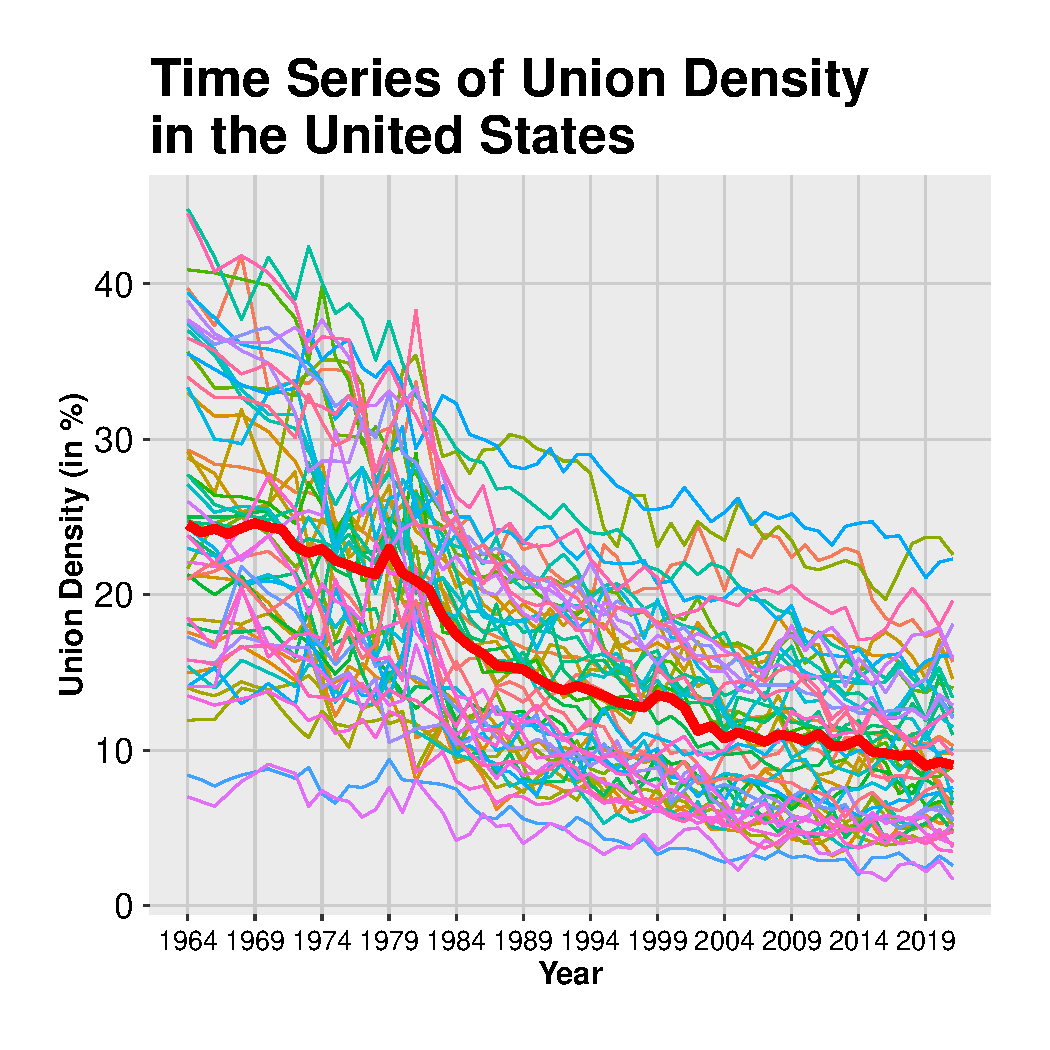
\includegraphics[width=.8\linewidth]{figure/TimesSeriesUnitedStates-1} 

}


\end{knitrout}
  \caption{detialed caption for figure } 
  \label{fig:usstatesuniondensity}
  \end{minipage}
\end{figure}

\begin{figure}[h]
\centering
\begin{minipage}{0.9\linewidth}
\begin{knitrout}
\definecolor{shadecolor}{rgb}{0.969, 0.969, 0.969}\color{fgcolor}\begin{kframe}


{\ttfamily\noindent\bfseries\color{errorcolor}{\#\# Error in `filter()`:\\\#\# i In argument: `!StateName \%in\% northern\_states`.\\\#\# Caused by error:\\\#\# ! object 'northern\_states' not found}}

{\ttfamily\noindent\bfseries\color{errorcolor}{\#\# Error in eval(expr, envir, enclos): object 'p2' not found}}\end{kframe}
\end{knitrout}

  \caption{[Detailed caption for Figure 2]}
  \label{fig:3}
  \end{minipage}
\end{figure}

\begin{figure}[h]
\centering
\begin{minipage}{0.9\linewidth}
\begin{knitrout}
\definecolor{shadecolor}{rgb}{0.969, 0.969, 0.969}\color{fgcolor}\begin{kframe}


{\ttfamily\noindent\bfseries\color{errorcolor}{\#\# Error in `filter()`:\\\#\# i In argument: `!StateName \%in\% southern\_states`.\\\#\# Caused by error:\\\#\# ! object 'southern\_states' not found}}

{\ttfamily\noindent\bfseries\color{errorcolor}{\#\# Error in eval(expr, envir, enclos): object 'p3' not found}}\end{kframe}
\end{knitrout}

  \caption{[Detailed caption for Figure 3]}
  \label{fig:4}
  \end{minipage}
\end{figure}

\begin{figure}[h]
\centering
\begin{minipage}{0.7\linewidth}
\begin{knitrout}
\definecolor{shadecolor}{rgb}{0.969, 0.969, 0.969}\color{fgcolor}

{\centering 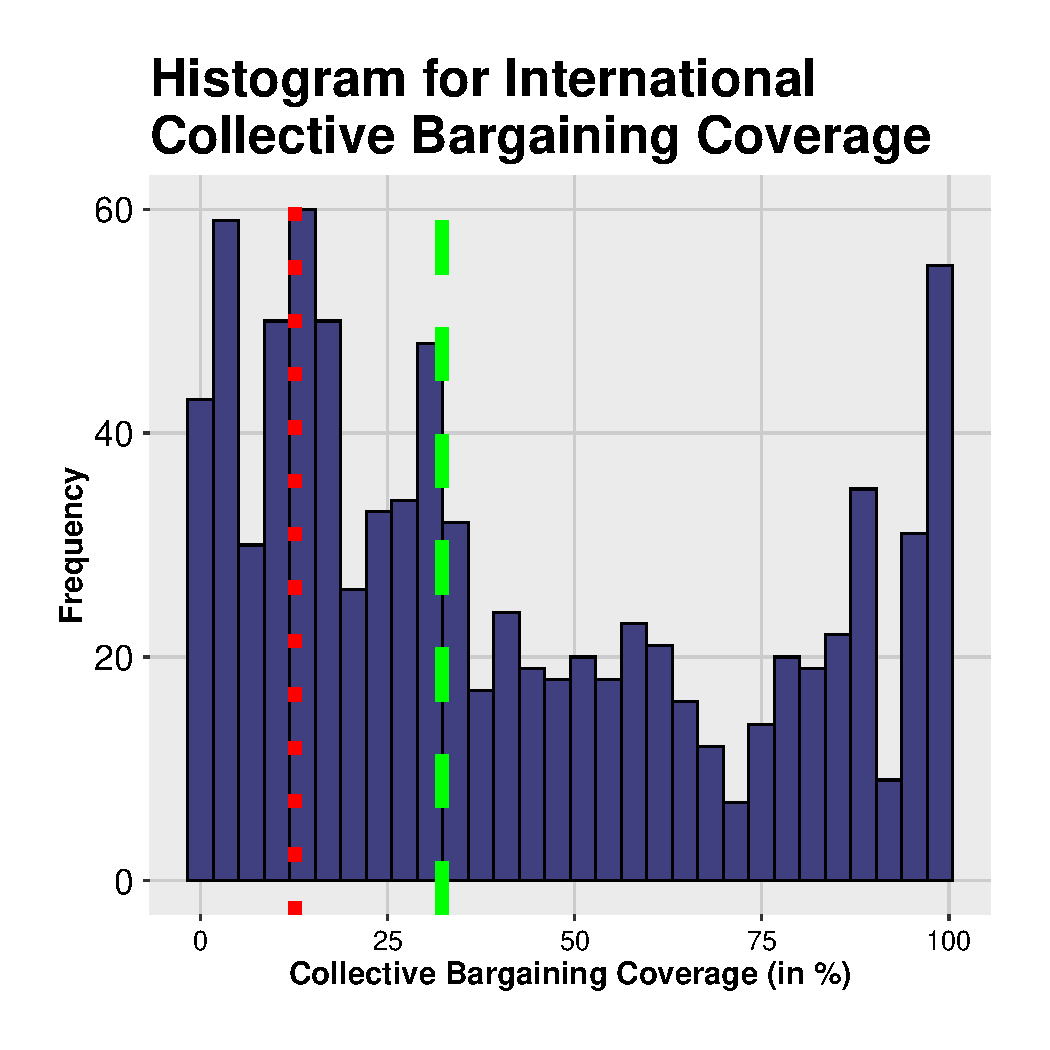
\includegraphics[width=0.7\linewidth]{figure/CollectiveBargaining-1} 

}


\end{knitrout}
  \caption[Collective Bargaining Coverage]{Histogram depicting the frequency distribution of collective bargaining coverage measured in percent recorded by the International Labor Organization database. The data is grouped by country, highlighting the predominance of collective bargaining coverage in the United States compared to the rest of the world.}
  \label{fig:5}
  \end{minipage}
\end{figure}
\hspace{5pt}
\begin{figure}[h]
\centering
  \begin{minipage}{0.7\linewidth}
\begin{knitrout}
\definecolor{shadecolor}{rgb}{0.969, 0.969, 0.969}\color{fgcolor}

{\centering 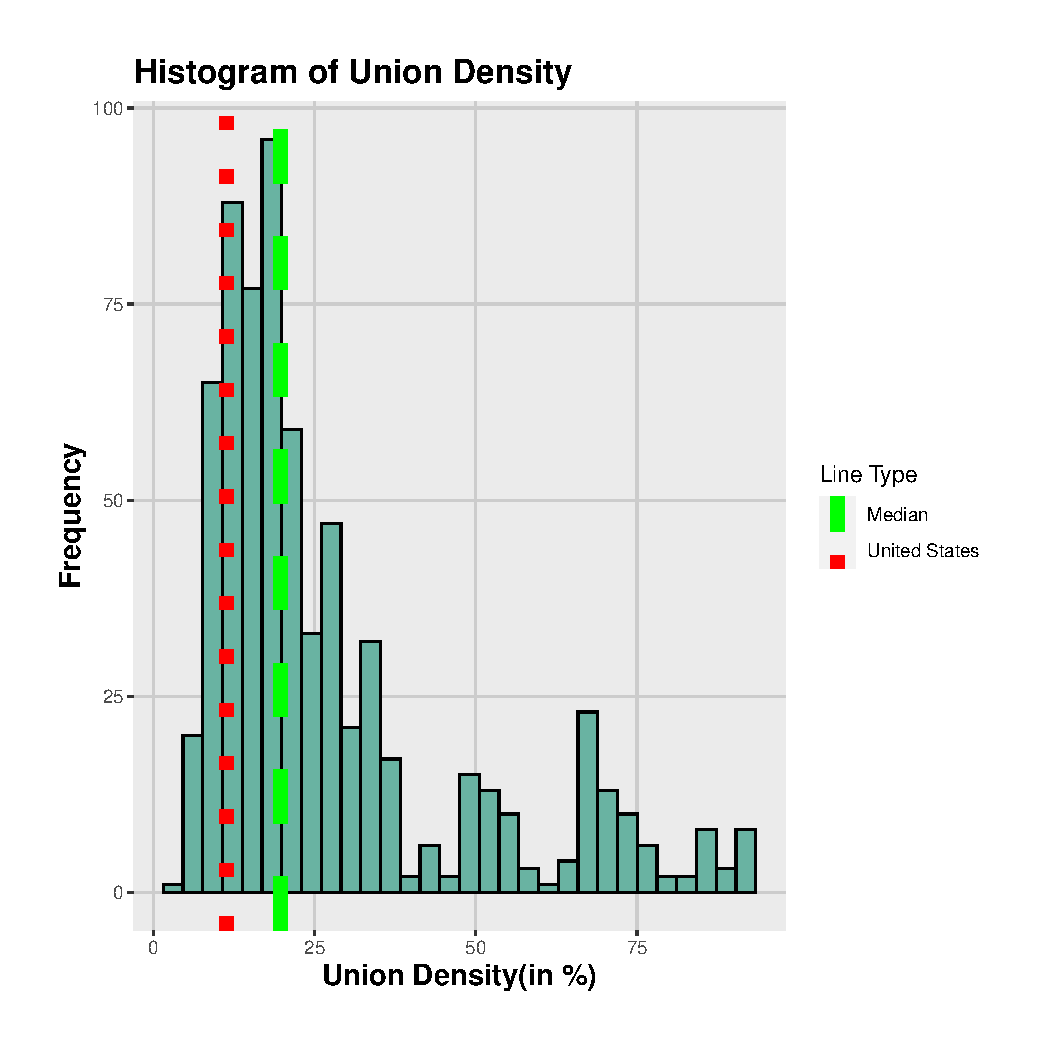
\includegraphics[width=0.7\linewidth]{figure/UnionDensity-1} 

}


\end{knitrout}
  \caption{Histogram depicting the frequency distribution of Union Density in percent. The percentage measures a country's total unionized industries; the higher the percentage, the more of that country's workforce is unionized. This data is grouped by country; the mean of the United States and the mean of the total population are marked on this graph.} 
  \label{fig:6}
  \end{minipage}
\end{figure}

\begin{figure}[h]
\centering
  \begin{minipage}{0.7\linewidth}
\begin{knitrout}
\definecolor{shadecolor}{rgb}{0.969, 0.969, 0.969}\color{fgcolor}

{\centering 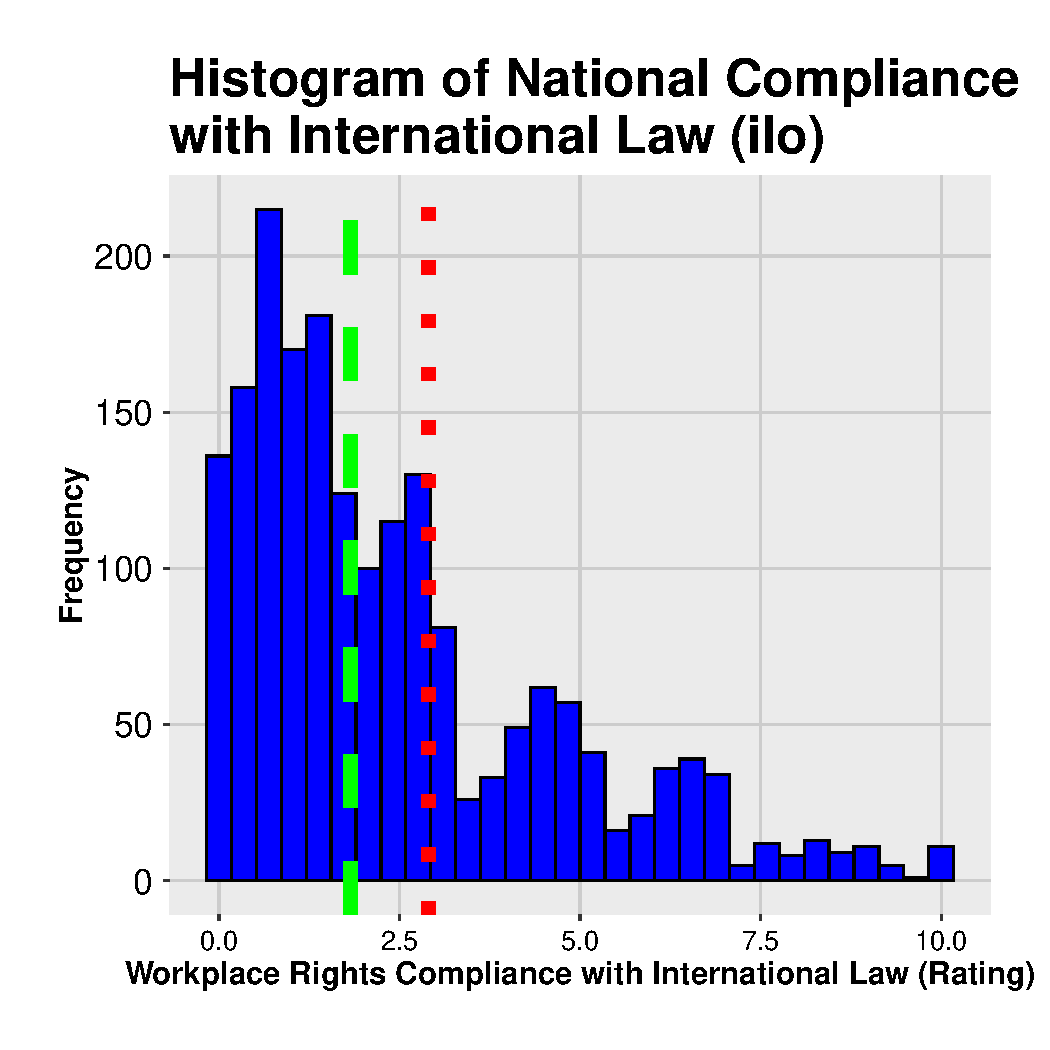
\includegraphics[width=0.7\linewidth]{figure/WorkplaceRights-1} 

}


\end{knitrout}
  \caption{Histogram depicting the frequency distribution of Compliance with international law bargaining coverage as scale from 0 to 10 with 10 being the most out of compliance with international law a country could be, and 0 being completely incompliance with international labor law recorded by the International Labor organization. This data is grouped by country, the united states place is marked in the along with the mean of all countries.}
  \label{fig:7}
  \end{minipage}
\end{figure}

\clearpage
%                                   United States
\section{Overview District of Columbia}
\begin{figure}[h!]
  \centering

  \begin{minipage}{0.48\linewidth}
\begin{knitrout}
\definecolor{shadecolor}{rgb}{0.969, 0.969, 0.969}\color{fgcolor}

{\centering 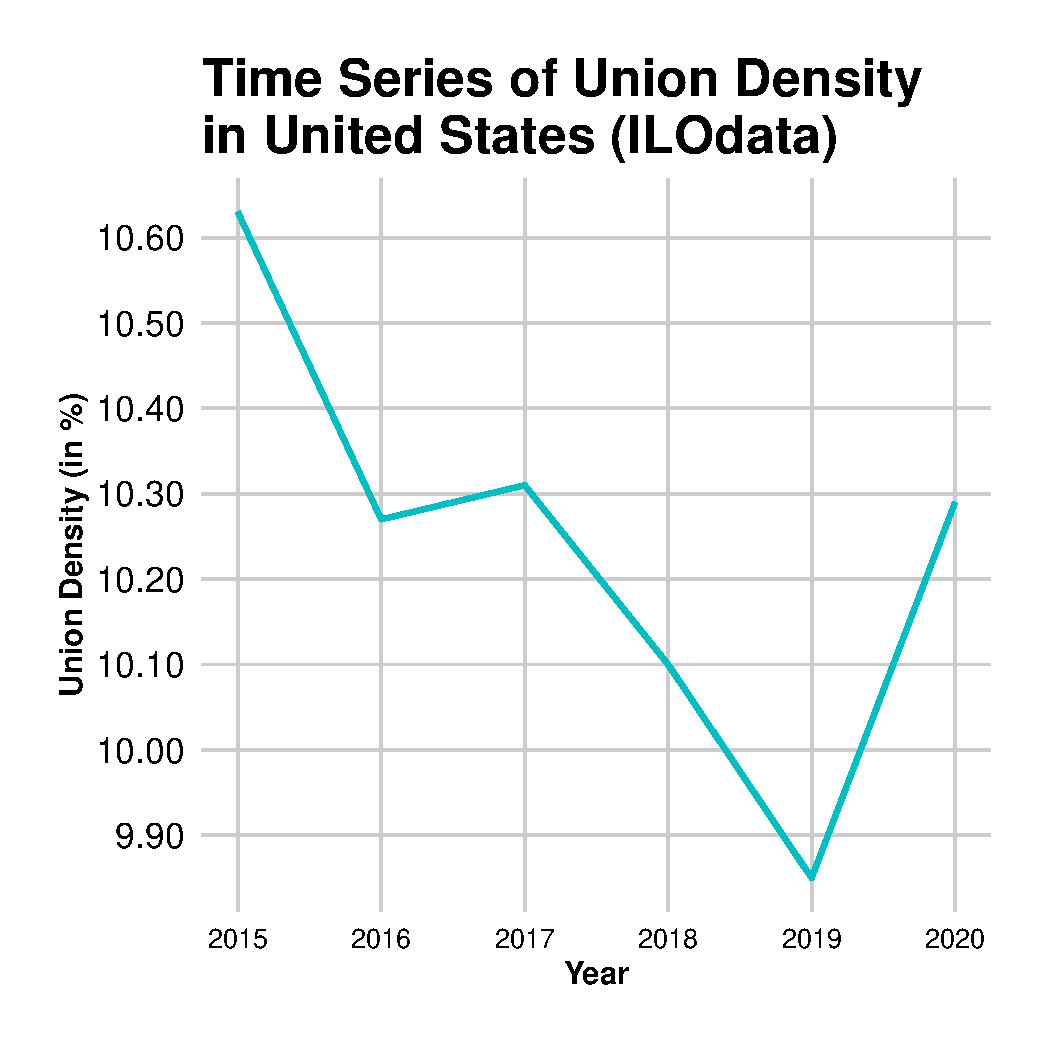
\includegraphics[width=0.7\linewidth]{figure/United_Statestradeuniondensity-1} 

}


\end{knitrout}
    \caption{Time Series chart depicting union density in United States from 2016 to 2017}
  \end{minipage}
  \hfill
  \begin{minipage}{0.48\linewidth}
\begin{knitrout}
\definecolor{shadecolor}{rgb}{0.969, 0.969, 0.969}\color{fgcolor}

{\centering 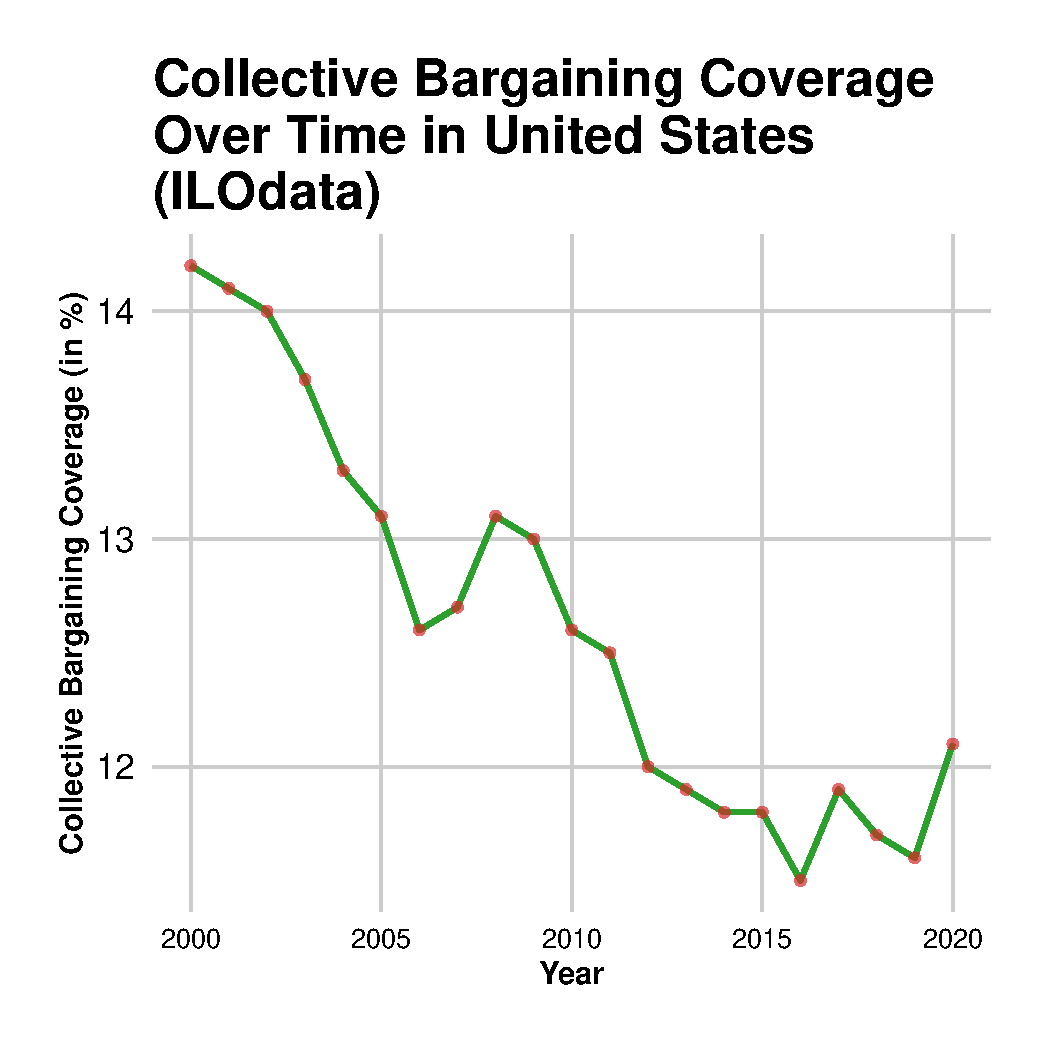
\includegraphics[width=0.7\linewidth]{figure/United_StatesCollectiveBargaining-1} 

}


\end{knitrout}
    \caption{Time Series chart of collective bargaining coverage...}
  \end{minipage}

 \begin{minipage}{0.48\linewidth}
\begin{knitrout}
\definecolor{shadecolor}{rgb}{0.969, 0.969, 0.969}\color{fgcolor}

{\centering 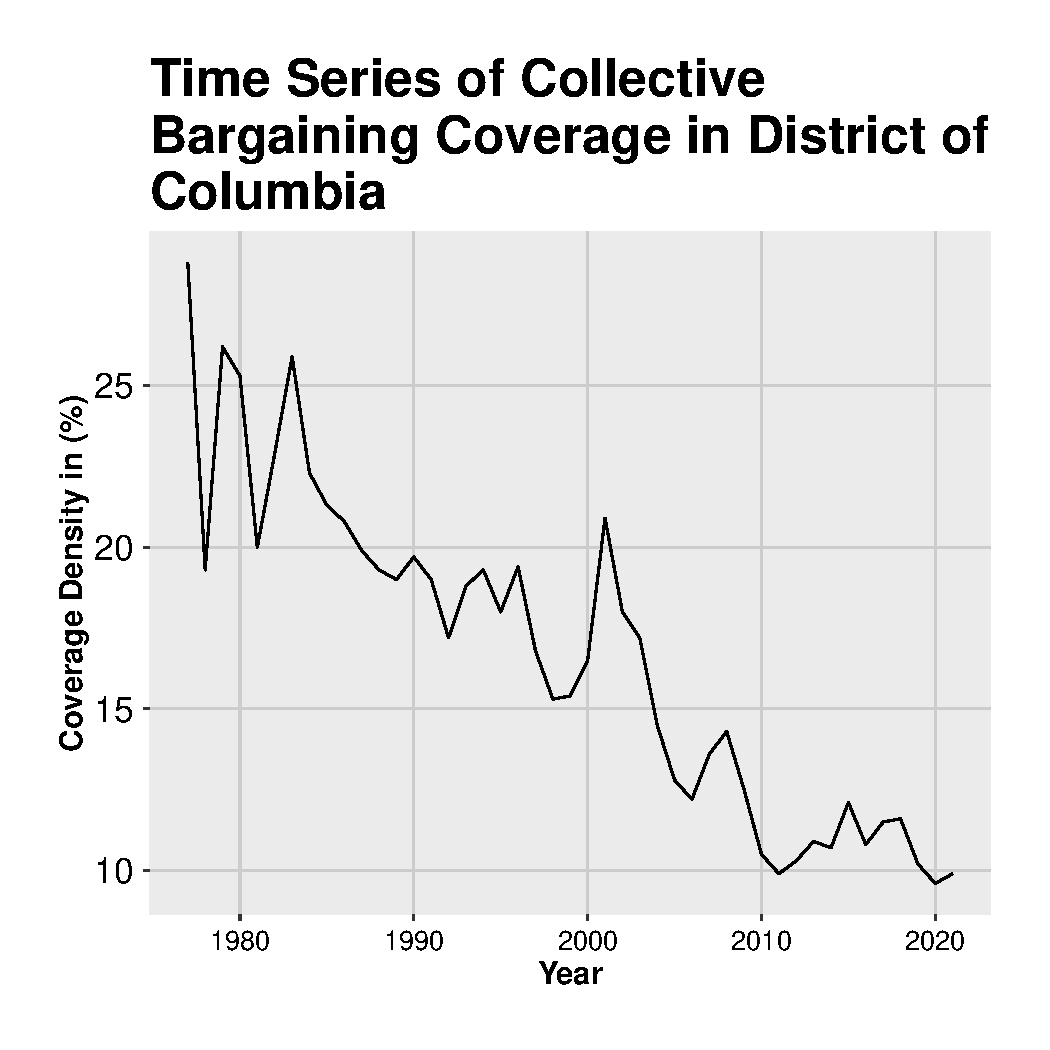
\includegraphics[width=0.7\linewidth]{figure/United_States_West_Virginia-1} 

}


\end{knitrout}
    \caption{Time series chart of Compliance with international law...}
 \end{minipage}
\hfill
  \begin{minipage}{0.48\linewidth}
\begin{knitrout}
\definecolor{shadecolor}{rgb}{0.969, 0.969, 0.969}\color{fgcolor}

{\centering 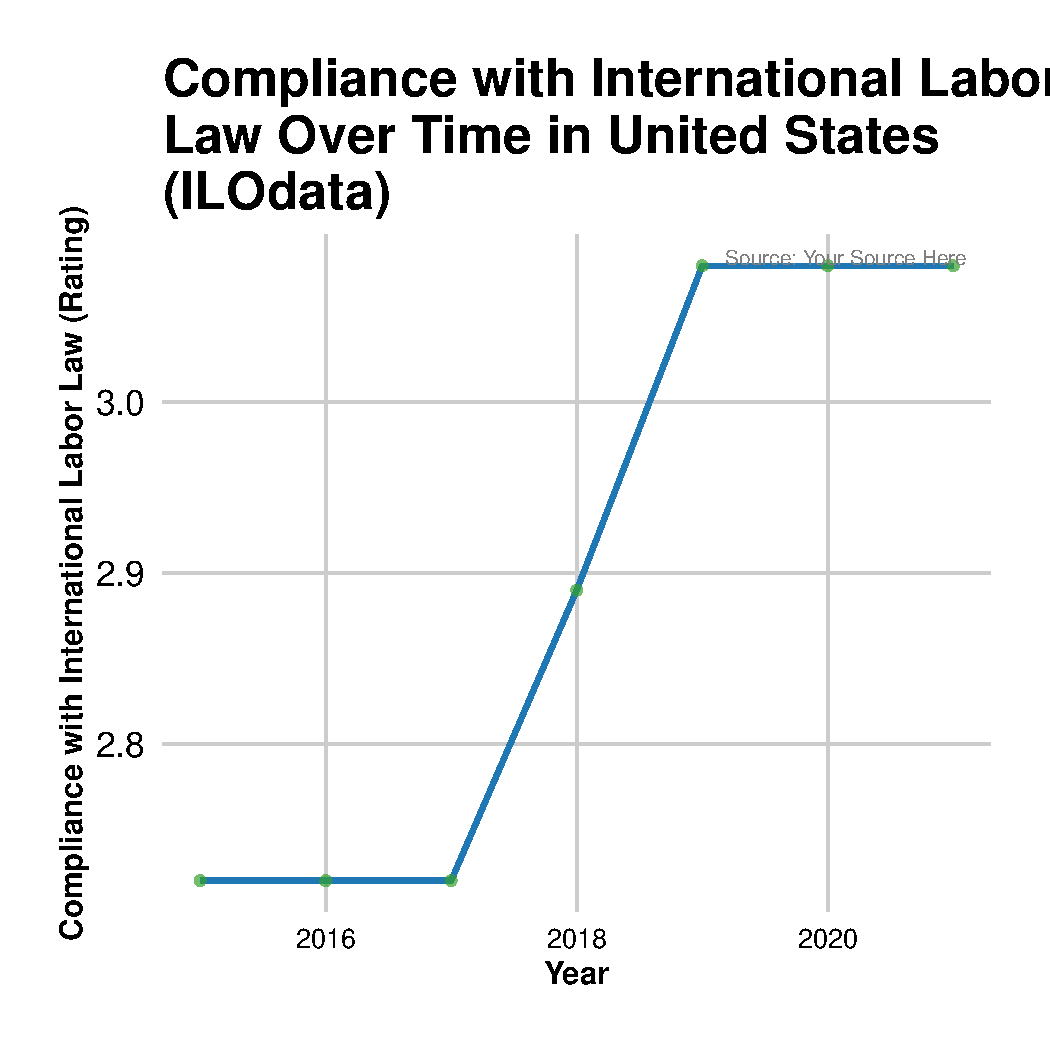
\includegraphics[width=0.7\linewidth]{figure/United_States_labor_compliance-1} 

}


\end{knitrout}
    \caption{Time series chart of Compliance with international law...}
  \end{minipage}
\end{figure}

\clearpage
%                                         China
% Top two charts side by side
\begin{figure}[h!]
  \centering
  \begin{minipage}{0.48\linewidth}
\begin{knitrout}
\definecolor{shadecolor}{rgb}{0.969, 0.969, 0.969}\color{fgcolor}

{\centering 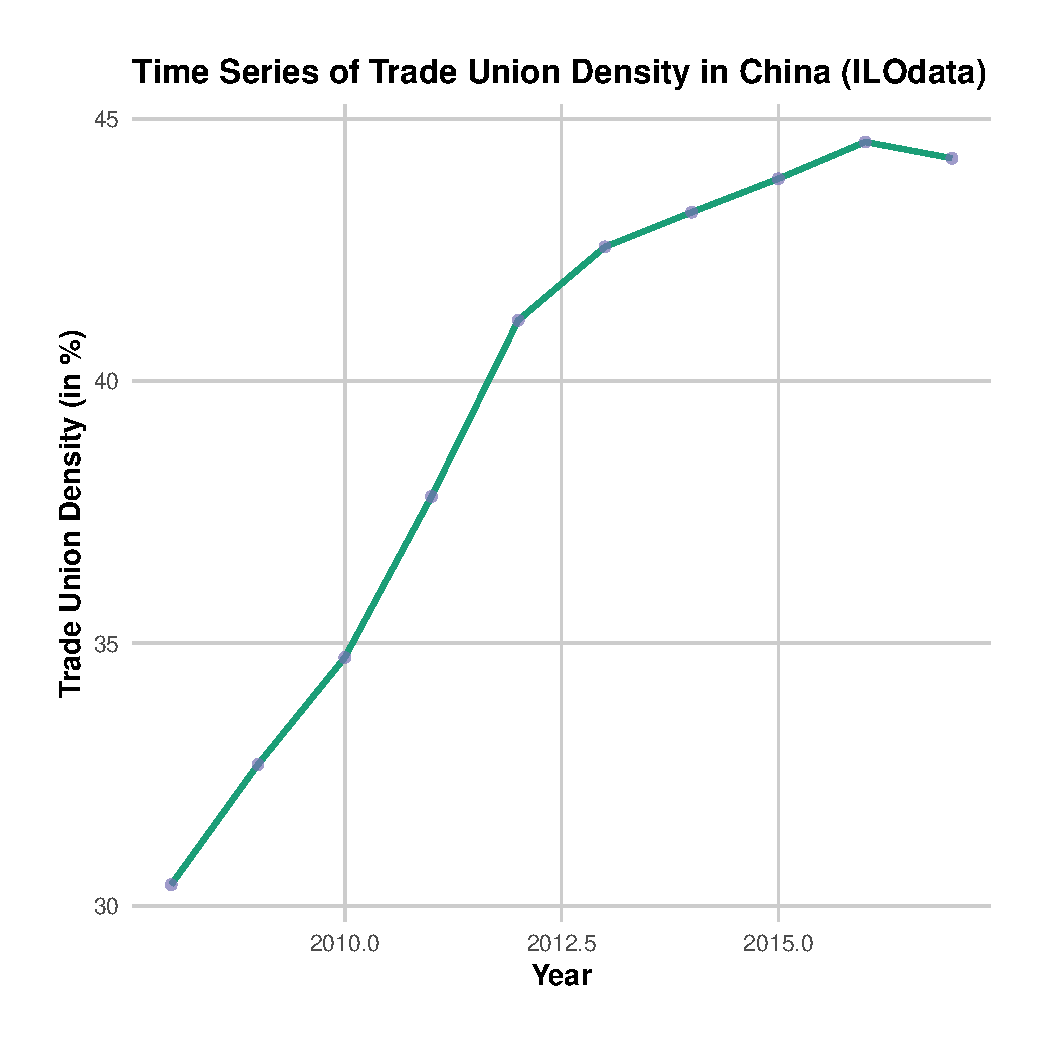
\includegraphics[width=0.7\linewidth]{figure/Chinatradeuniondensity-1} 

}


\end{knitrout}
    \caption{Time Series chart depicting union density in China from 2016 to 2017}
    \label{fig:union-density-china}
  \end{minipage}
  \hfill % Space between the two minipages
  \begin{minipage}{0.48\linewidth}
\begin{knitrout}
\definecolor{shadecolor}{rgb}{0.969, 0.969, 0.969}\color{fgcolor}

{\centering 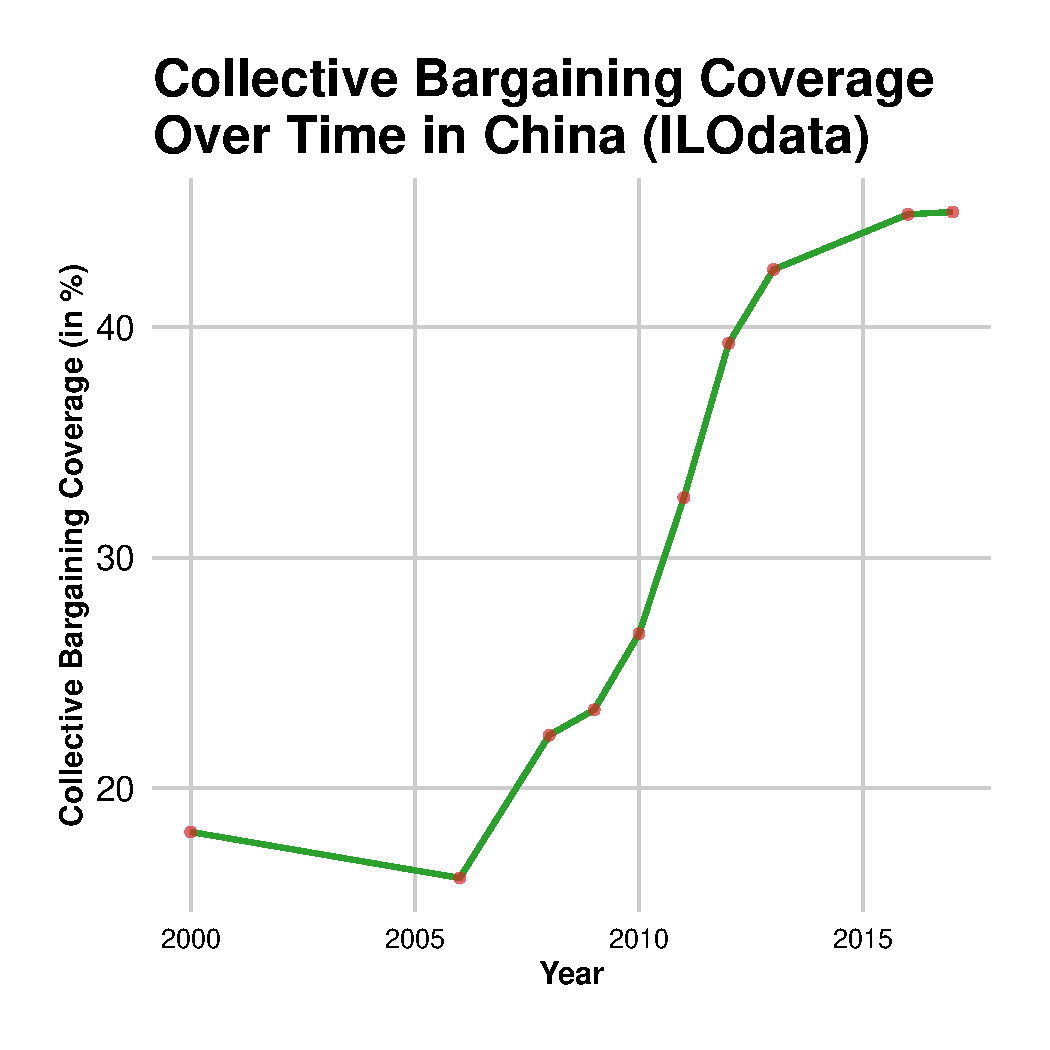
\includegraphics[width=0.7\linewidth]{figure/ChinaCollectiveBargaining-1} 

}


\end{knitrout}
    \caption{Time Series chart of collective bargaining coverage...}
    \label{fig:china-collective-bargaining}
  \end{minipage}
\end{figure}

% Third chart below
\begin{figure}[h!]
  \centering
  \begin{minipage}{0.6\linewidth}
\begin{knitrout}
\definecolor{shadecolor}{rgb}{0.969, 0.969, 0.969}\color{fgcolor}

{\centering 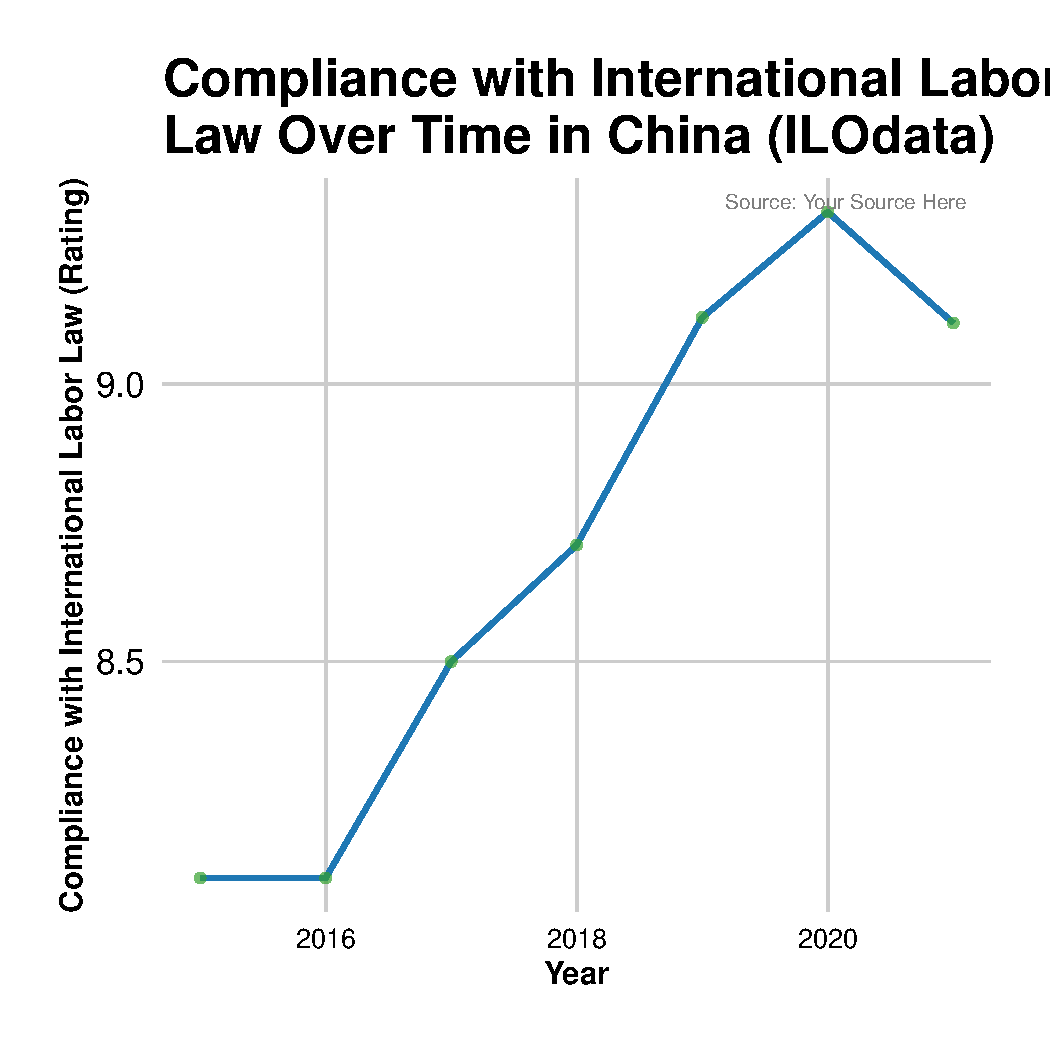
\includegraphics[width=0.7\linewidth]{figure/China_labor_compliance-1} 

}


\end{knitrout}
    \caption{Time series chart of Compliance with international law...}
    \label{fig:labor-compliance-china}
  \end{minipage}
\end{figure}


\clearpage
\begin{figure}[h]
\centering
  \begin{minipage}{0.7\linewidth}
  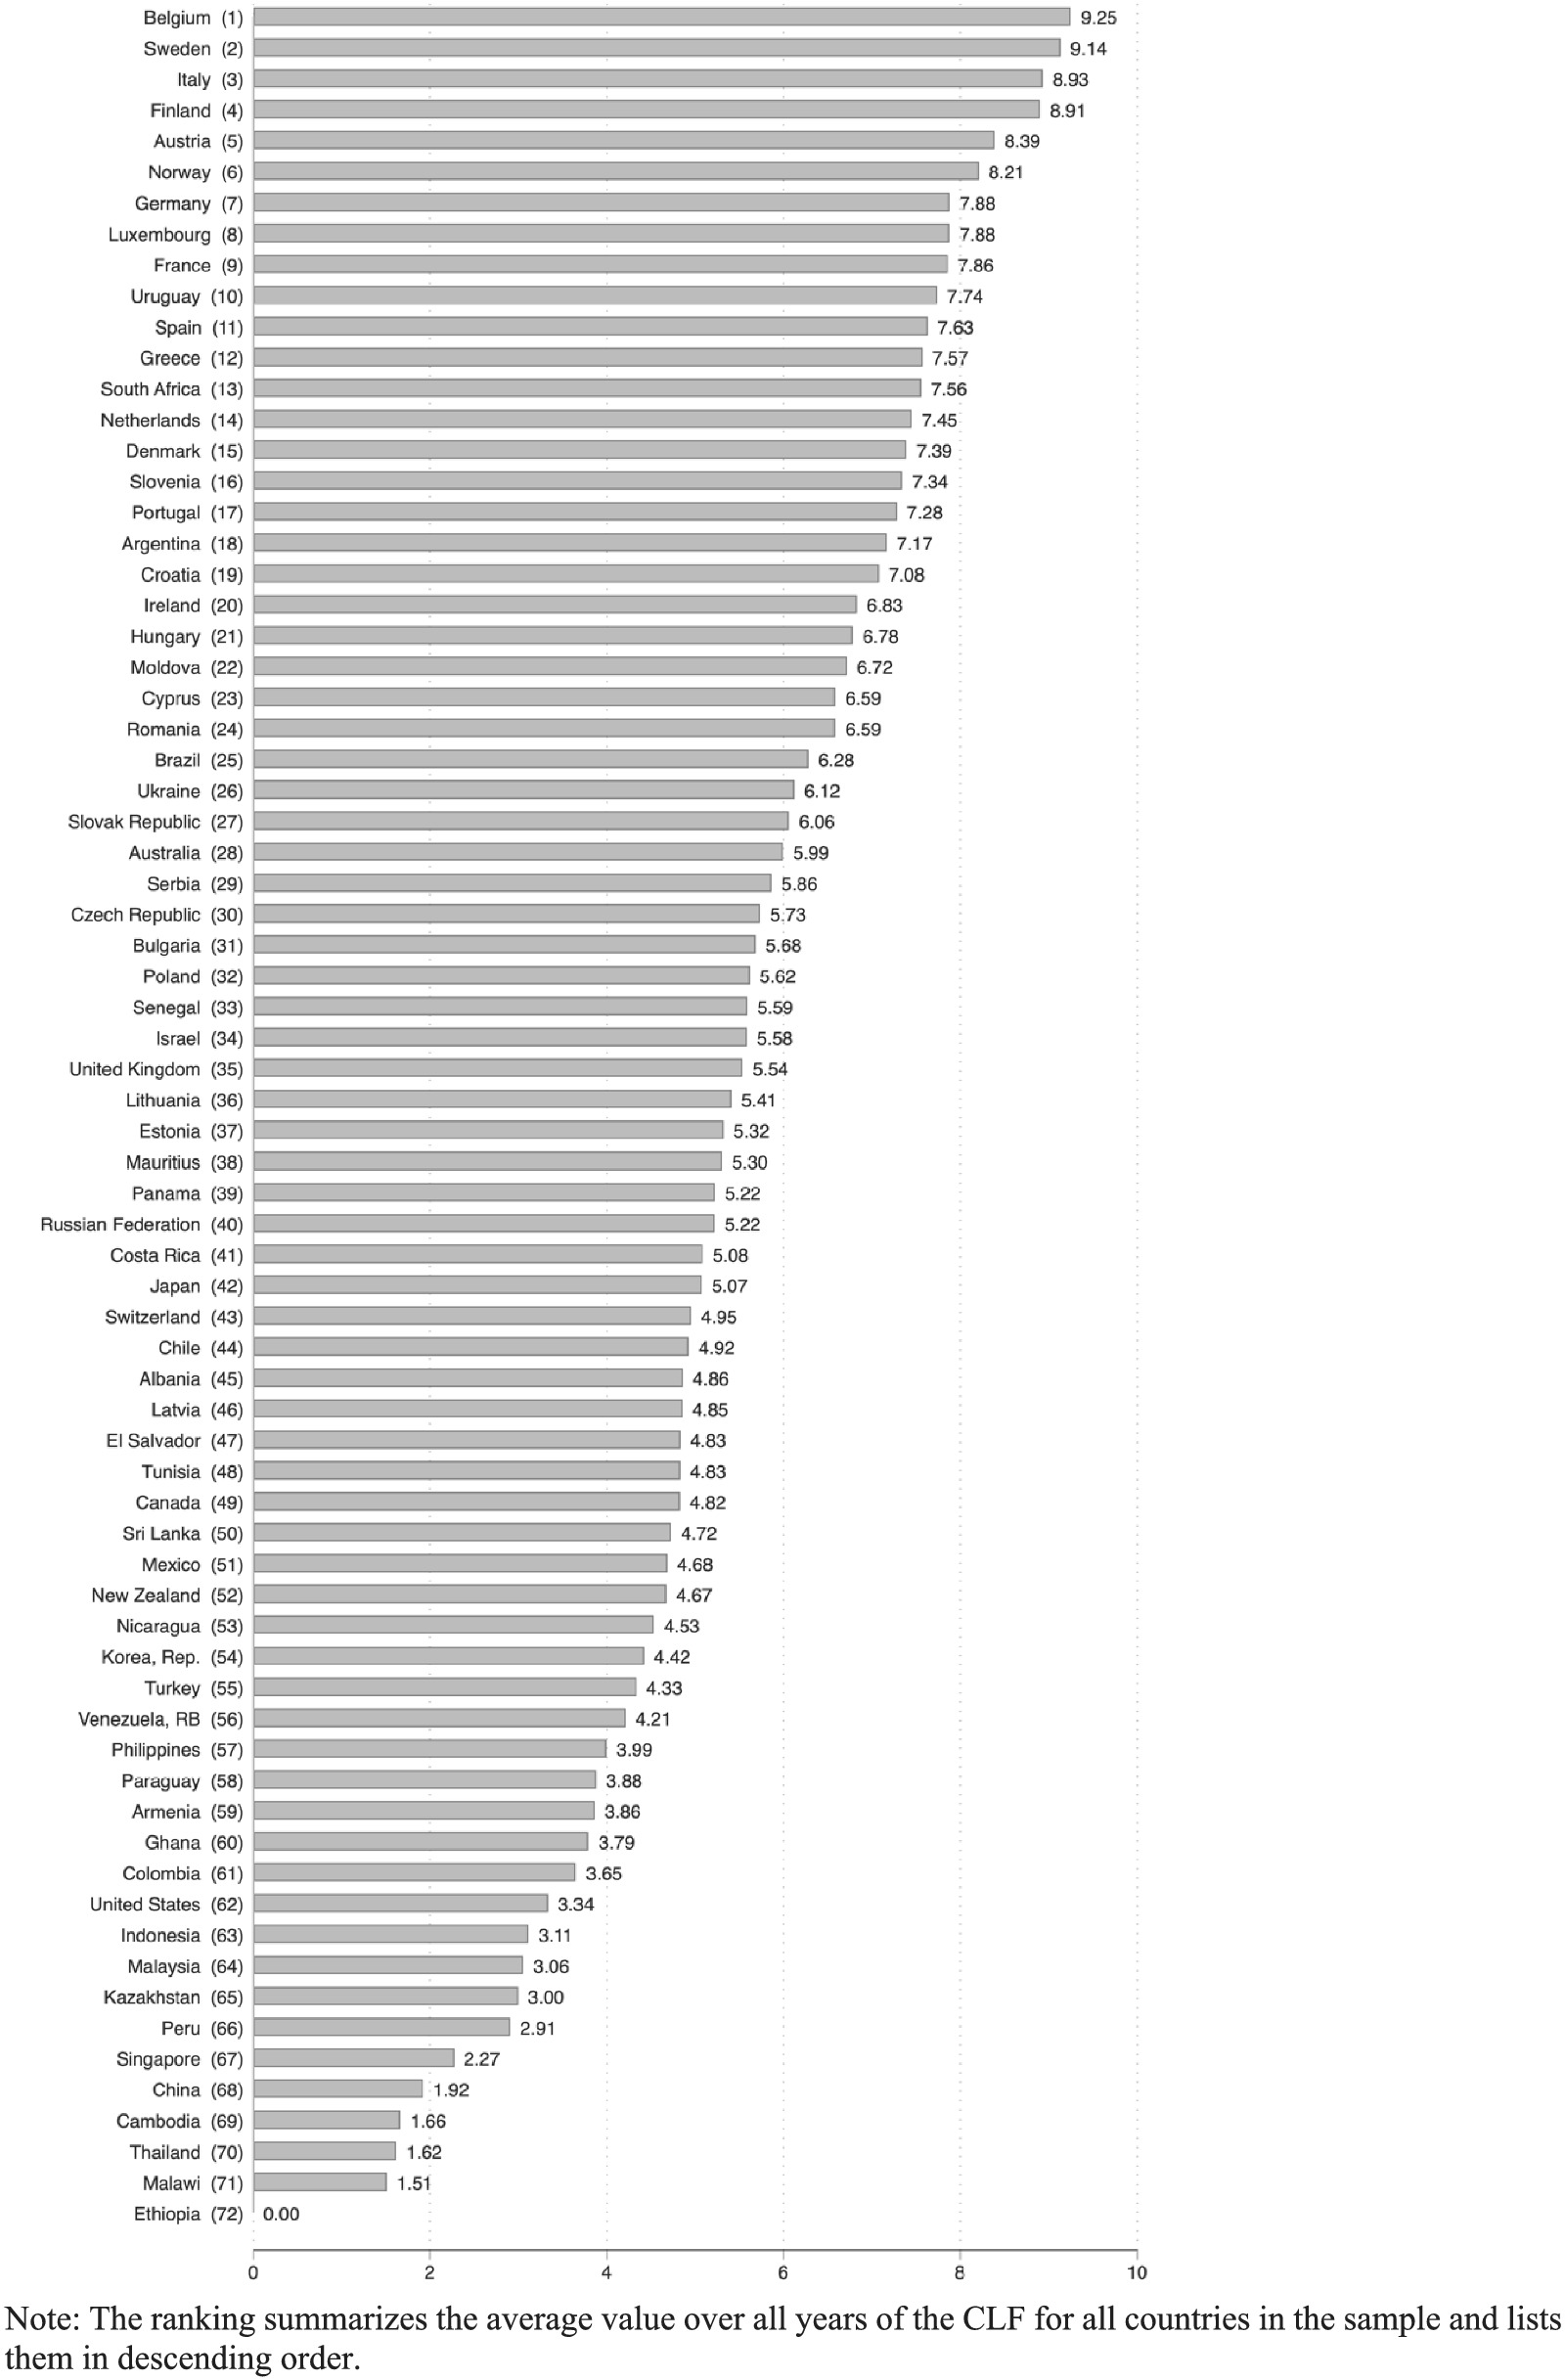
\includegraphics[width=\linewidth]{~/Lab2/graphs/udstudfy.jpg}
  \caption{Histogram depicting the distribution of the collective labour force index. The incomplete data availability pushes the Index down to around 72 countries, so the ranking matters less than the Index itself. The picture it paints is the freedom a working person has in the labor force(Union Power). This study is an assessment of union power. It indicates union power by combining and weighing the following stats: Trade Union Density, Collective Bargaining Coverage, Labour Force Participation Rate, Employment in agriculture, Democracy, Core labor rights ratification, hiring and firing constraints, and Hours Regulation. The United States is 62(3.32 index rating) in the Index, and China's place is 68 (1.92 index rating). The data is only recorded from 2010 to 2016. }
  \label{fig:1}
  \end{minipage}
\end{figure}


\clearpage
\section{Conclusion}
Summarize the main findings and their relevance to the initial objectives of your study.

\clearpage

\section*{References}
\begin{enumerate}
  \item Visser, J. (2021). OECD/AIAS database on Institutional Characteristics of Trade Unions, Wage Setting, State Intervention and Social Pacts (ICTWSS) [Data set]. OECD. Retrieved from \url{https://www.oecd.org/employment/ictwss-database.htm}
  
  \item International Labour Organization. (2022). Trade union density rate () [Data set]. Industrial Relations Data (IRdata). Retrieved from \url{https://www.ilo.org/shinyapps/bulkexplorer30/?lang=en\&id=ILR\_TUMT\_NOC\_RT\_A}
  
  \item International Labour Organization. (2022). Collective bargaining coverage rate () [Data set]. Industrial Relations Data (IRdata). Retrieved from \url{https://www.ilo.org/shinyapps/bulkexplorer36/?lang=en\&id=ILR\_CBCT\_NOC\_RT\_A}
  
  \item International Labour Organization. (2023). SDG indicator 8.8.2 - Level of national compliance with labour rights (freedom of association and collective bargaining) based on ILO textual sources and national legislation[Data set]. SDG Labour Market Indicators (ILOSDG). Retrieved from \url{https://www.ilo.org/shinyapps/bulkexplorer30/?lang=en\&id=ILR\_TUMT\_NOC\_RT\_A}
  
  \item Palley, T. I., \& LaJeunesse, R. M. (2007). Social attitudes, labor law, and union organizing: Toward a new economics of union density. \textit{Journal of Economic Behavior and Organization}, 62(2), 237–254. \url{https://doi.org/10.1016/j.jebo.2005.02.003}
  
  \item Dollard, M. F., \& Neser, D. Y. (2013). Worker health is good for the economy: Union density and psychosocial safety climate as determinants of country differences in worker health and productivity in 31 European countries. \textit{Social Science \& Medicine}, 92, 114–123. \url{https://doi.org/10.1016/j.socscimed.2013.04.028}
  
  \item Normann, H. E., \& Tellmann, S. M. (2021). Trade unions' interpretation of a just transition in a fossil fuel economy. \textit{Environmental Innovation and Societal Transitions}, 40, 421–434. \url{https://doi.org/10.1016/j.eist.2021.09.007}
  
  \item Flavin, P., \& Radcliff, B. (2011). Labor union membership and voting across nations. \textit{Electoral Studies}, 30(4), 633–641. \url{https://doi.org/10.1016/j.electstud.2011.06.001}
  
  \item McFarland, S. (2019). Spatialities of class formation: Urban sprawl and union density in U.S. metropolitan areas. \textit{Geoforum}, 102, 86–96. \url{https://doi.org/10.1016/j.geoforum.2019.03.015}
\end{enumerate}


\end{document}
